\documentclass[11pt]{ctexart}
% \documentclass{article}
\textheight 23.5cm \textwidth 15.8cm
%\leftskip -1cm
\topmargin -1.5cm \oddsidemargin 0.3cm \evensidemargin -0.3cm

\usepackage{verbatim}
\usepackage{fancyhdr}
\usepackage{graphicx}
\usepackage{amssymb}
\usepackage{amsmath}
\usepackage{booktabs}
\usepackage{subcaption}
\usepackage{listings}
\usepackage{color}
\usepackage{geometry}


\definecolor{mygreen}{rgb}{0,0.6,0}
\definecolor{mygray}{rgb}{0.5,0.5,0.5}
\definecolor{mymauve}{rgb}{0.58,0,0.82}

\lstset{
  language=Matlab,                % 设定语言为MATLAB
  frame=single,                   % 外围框架
  basicstyle=\footnotesize\ttfamily,   % 基本代码风格
  keywordstyle=\color{blue},      % 关键词风格
  commentstyle=\color{mygreen},   % 注释风格
  stringstyle=\color{mymauve},    % 字符串风格
  numbers=left,                   % 行号位置
  numberstyle=\tiny\color{mygray}, % 行号风格
  stepnumber=1,                   % 行号步长
  numbersep=5pt,                  % 行号与代码间隔
  backgroundcolor=\color{white},  % 代码背景色
  showspaces=false,               % 不显示空格
  showstringspaces=false,         % 不显示字符串中的空格
  showtabs=false,                 % 不显示制表符
  tabsize=4,                      % 制表符宽度
  captionpos=b,                   % 标题位置
  breaklines=true,                % 自动换行
  breakatwhitespace=false,        % 仅在空格处换行
  escapeinside={\%*}{*)},         % 可以添加LaTeX内容
}


\ctexset {
     section/format    += \sffamily\raggedright,
     subsection/format += \fbox,
}


\title{FEM Code Report3 - 2nd Order}
\author{SA24229016 王润泽}

\begin{document}
\maketitle

\section{Introduction}
编写程序求解两点边值问题:
\begin{equation}
     \begin{aligned}
          -u'' &= f, \quad 0 < x < 1, \\
          u(0) &= u(1) = 0.
     \end{aligned}
\end{equation}
选取等距网格剖分,有限元空间选取分段二次多项式空间 $ V_h $ ,每个单元的基函数利用单元 $ I_j = [x_{j-1},x_j] $ 端点 $ x_{j-1}, x_j $ 和中点 $ x_{j-1/2} =  \frac{x_{j-1} + x_j}{2} $ 得到。

\section{Method}
\subsection{Variational Formulation}
对于问题(1),转换成变分问题为:求 $ u \in V= \{ v \in H^1(0,1) : v(0) = v(1) = 0 \} $ ,使得对于所有 $ v \in V $ ,有:
\begin{equation}
     a(u,v) = (f,v), \quad \forall v \in V,
\end{equation}
其中 $ a(u,v) = \int_0^1 u'v' \, dx $ , $ (f,v) = \int_0^1 fv \, dx $ 。

\subsection{基函数}
实验中采用等距网格划分,单元数为 N,节点处的值为 $ u_i$ , 步长$h_i = x_{i}-x_{i-1}=h$ 。选取分片二次全局基函数$ \phi_i(x) $,并选取其张成的有限维二次空间 $ V_h $ 进行求解。

对于标准单元 $ I = [0,1] $, 其标准单元型基函数定义如下:
\begin{equation}
     \varphi^0(x) = \left\{
     \begin{aligned}
          &(2x-1)(x-1) , \quad x \in [0,1], \\
          &0, \quad \text{otherwise}.
     \end{aligned}
     \right.
\end{equation}

\begin{equation}
     \varphi^1(x) = \left\{
     \begin{aligned}
          &4x(1-x) , \quad x \in [0,1], \\
          &0, \quad \text{otherwise}.
     \end{aligned}
     \right.
\end{equation}

\begin{equation}
     \varphi^2(x) = \left\{
     \begin{aligned}
          &(2x-1)x , \quad x \in [0,1], \\
          &0, \quad \text{otherwise}.
     \end{aligned}
     \right.
\end{equation}

对于单元 $ I_i = [x_{i-1},x_i] $,其局部基函数 $ \psi $ 定义如下:
\begin{equation}
     \psi^0_i(x) = \varphi^0\left(\frac{x-x_{i-1}}{h_i}\right)
\end{equation}
\begin{equation}
     \psi^1_i(x) = \varphi^1\left(\frac{x-x_{i-1}}{h_i}\right)
\end{equation}
\begin{equation}
     \psi^2_i(x) = \varphi^2\left(\frac{x-x_{i-1}}{h_i}\right)
\end{equation}

对每个节点 $ x_i,x_{i-1/2} $ ,一共有 $ 2N+1 $个对应的全局基函数 $ \phi $,定义如下:
\begin{equation}
     \phi_{i} = \psi^2_{i}+\psi^0_{i+1} =\left\{
          \begin{aligned}
               &\left(2\frac{x-x_{i-1}}{h_i}-1\right)\left(\frac{x_i-x}{h_i}\right),& \quad x \in I_i, \\
               &\left(2\frac{x_{i+1}-x}{h_{i+1}}-1\right)\left(\frac{x_{i+1}-x}{h_{i+1}}\right),& \quad x \in I_{i+1}, \\     
               &0,& \quad \text{otherwise}. 
          \end{aligned}
     \right.
\end{equation}
\begin{equation}
     \phi_{i-1/2} = \psi^1_{i}= \left\{
          \begin{aligned}
               &4\left(\frac{x-x_{i-1}}{h_i}\right)\left(\frac{x_i-x}{h_i}\right),& \quad x \in I_i, \\
               &0,& \quad \text{otherwise}.
          \end{aligned}
     \right.
\end{equation}



全局基函数形状如图1所示。由此可以得到由二次基函数张成的有限维空间 $ V_h $所定义的带解函数:
\begin{equation}
     u_h = \sum_{i=1}^{N-1} u_i \phi_i + \sum_{i=1}^{N} u_{i-1/2} \phi_{i-1/2}
\end{equation}
其中,$ u_i, u_{i-1/2} $ 为待求解的系数。

\begin{figure}[htbp]
     \centering
     \begin{subfigure}{0.4\textwidth}
          \centering
          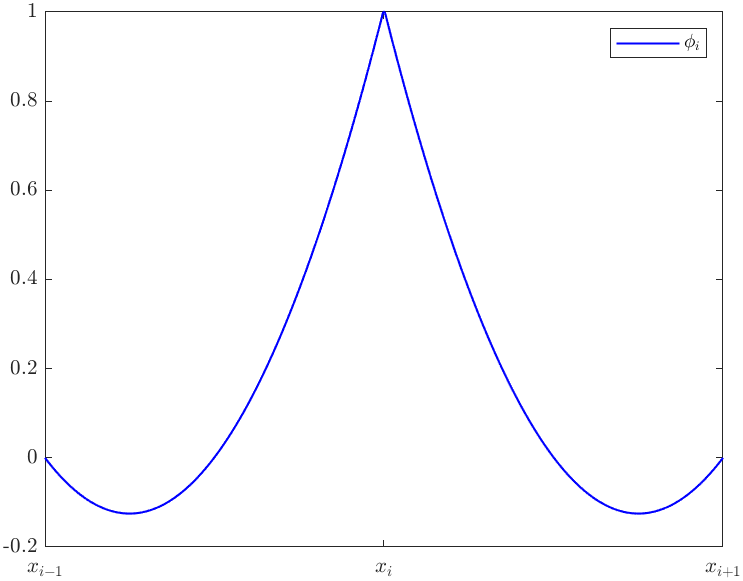
\includegraphics[width=0.9\linewidth]{phi_i.png}
     \end{subfigure}
     \begin{subfigure}{0.4\textwidth}
          \centering
          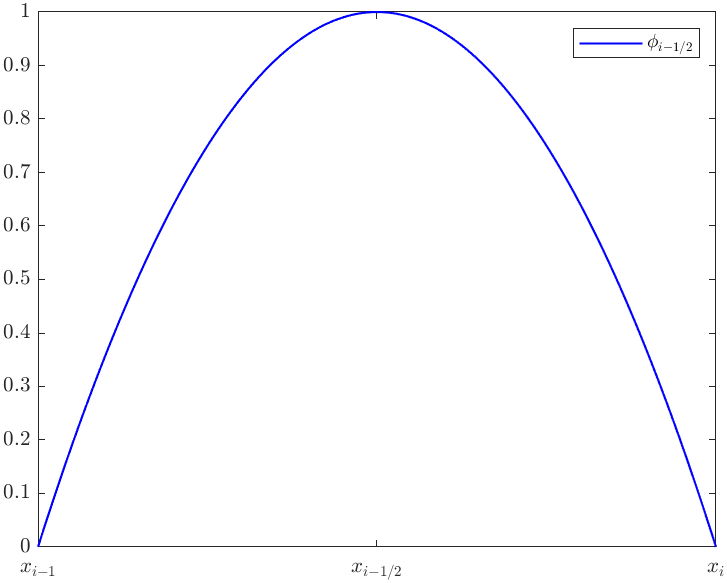
\includegraphics[width=0.9\linewidth]{phi_12.png}
     \end{subfigure}
     \caption{全局基函数}
\end{figure}

\subsection{刚度矩阵}
局部刚度矩阵的系数为:
\begin{equation}
     K_{l,m}= \int_{I_i} \psi^l_i(x)'\psi^m_i(x)' \, dx = \int_{0}^{1} \phi^l(x)'\phi^m(x)' \, dx, \quad l,m = 0,1,2.
\end{equation}

计算可得:
\begin{equation}
     K =\frac{1}{h}
     \begin{pmatrix}
          \frac{7}{3}, & -\frac{8}{3}, & \frac{1}{3} \\
          -\frac{8}{3}, & \frac{16}{3}, & -\frac{8}{3} \\
          \frac{1}{3}, & -\frac{8}{3}, & \frac{7}{3}
     \end{pmatrix}
\end{equation}

全局刚度矩阵:
\begin{equation}
     A = \frac{1}{h}
     \begin{pmatrix}
          \frac{16}{3} & -\frac{8}{3} & 0 & 0 & \cdots & 0 & 0\\
          -\frac{8}{3} & \frac{14}{3} & -\frac{8}{3} &\frac{1}{3} &\cdots & 0 & 0\\
          0 & -\frac{8}{3} & \frac{16}{3} & -\frac{8}{3} & \cdots & 0 & 0\\
          0 & \frac{1}{3} & -\frac{8}{3} & \frac{14}{3} & \cdots & 0 & 0\\
          \vdots & \vdots & \vdots & \vdots & \ddots & \vdots & \vdots\\
          0 & 0 & 0 & 0 & \cdots & \frac{14}{3} & -\frac{8}{3}\\
          0 & 0 & 0 & 0 & \cdots & -\frac{8}{3} & \frac{16}{3}
     \end{pmatrix}
     \in \mathbb{R}^{(2N-1) \times (2N-1)}
\end{equation}

\subsection{荷载向量}
对于荷载向量 $ F $ 的分量计算为 $ f_i = (f,\phi_i) $ ,$ f_{i-1/2} = (f,\phi_{i-1/2}) $,Taylor展开近似计算可得:
\begin{equation}
     \begin{aligned}
          f_i &\approx \frac{1}{3} hf(x_i)\\
          f_{i-1/2} &\approx \frac{2}{3} hf(x_{i-1/2})
     \end{aligned}
\end{equation}

\subsection{数值解}
对于离散问题,只需求解 $ AU = F $ 即可得到 $ U $,即为问题 (1) 的数值解,其中:
\begin{equation}
     U= \begin{pmatrix}
          u_{1/2}\\
          u_1\\
          \vdots\\
          u_{N-1}\\
          u_{N-1/2}
     \end{pmatrix}, \quad
     F= \begin{pmatrix}
          f_{1/2}\\
          f_1\\
          \vdots\\
          f_{N-1}\\
          f_{N-1/2}
     \end{pmatrix}
\end{equation}

\section{Results}

实验中选择 $ f(x) = 2\pi^2\sin(\pi x) $ 作为右端项,$ u(x) = \sin(\pi x) $ 作为精确解。取 $ N = 10,20,40,80 $,分别计算 $ L^2 $ 误差和 $ H^1 $ 误差。

对于求得的系数,先进行插值,然后进行梯形公式数值积分。实验得到的结果如表1,可以看出在二次多项式空间下,有限元方法的 $ L^2 $ 误差是三阶的,$ H^1 $ 误差是二阶的

% Table generated by Excel2LaTeX from sheet 'Sheet1'
\begin{table}[htbp]
     \centering
	\caption{误差分析}
	  \begin{tabular}{|c|cc|cc|}
	  \toprule
	  N     & \multicolumn{1}{c}{$L^2$ error} & \multicolumn{1}{c|}{order} & \multicolumn{1}{c}{$H^1$ error} & \multicolumn{1}{c|}{order} \\
       \midrule
       10    & 1.63E-03 &       & 8.03E-06 &  \\
       20    & 4.12E-04 & 3.00 & 1.00E-06 & 1.98 \\
       40    & 1.03E-04 & 3.00 & 1.25E-07 & 2.00 \\
       80    & 2.56E-05 & 3.00 & 1.56E-08 & 2.01 \\   
       \bottomrule
       \end{tabular}%
       \label{tab:error}%
\end{table}%
\section{Discussion}
根据误差方程:
\begin{equation}
     <u-u_h,v> = 0, \quad \forall v \in V_h
\end{equation}

等价于:
\begin{equation}
     || u-u_h || \le || u-v ||, \quad \forall v \in V_h
\end{equation}

假设 $ u_I $ 是 $ u $ 的分片二次插值函数,在区间 $ [a,b] $上,满足:
\begin{equation}
     u(a) = u_I(a), \quad u(b) = u_I(b), \quad u(\frac{a+b}{2}) = u_I(\frac{a+b}{2})
\end{equation}

定义函数 $ f(x) = u(x) - u_I(x) $,那么 $ f(a) = f(b) = f(\frac{a+b}{2}) = 0 $,由微分中值定理可得:f'(x) 在区间 $ [a,b] $ 上至少有两个零点,即 $ f''(x) $ 在区间 $ [a,b] $ 上至少有一个零点。 因此可以得到:
\begin{equation}
     \begin{aligned}
          \sup|f''| &< C(b-a)M, \\
          \sup|f'| &< C(b-a)^2M\\
          \sup|f| &< C(b-a)^3M
     \end{aligned}
\end{equation}
其中, $ M = \sup|u''| $ , $ C $ 为常数。

由此可知,对于每个区间 $ I_i $,有:
\begin{equation}
     \int_{I_i} |u-u_h|^2 \, dx \le C h^7M\\
     \int_{I_i} |u'-u_h'|^2 \, dx \le C h^5M
\end{equation}

对于整个区间 $ [0,1] $,有:
\begin{equation}
     \begin{aligned}
          ||u-u_h||^2 &\le C h^6M\\
          ||u'-u_h'||^2 &\le C h^4M
     \end{aligned}
\end{equation}

由此可以证明,对于二次多项式空间,有限元方法的 $ L^2 $ 误差是三阶的,$ H^1 $ 误差是二阶的:
\begin{equation}
     \begin{aligned}
          ||u-u_h|| = O(h^3)\\
          ||u'-u_h'|| = O(h^2)
     \end{aligned}
\end{equation}

\end{document}